\documentclass[conference]{IEEEtran}
\IEEEoverridecommandlockouts
\usepackage{cite}
\usepackage[utf8]{inputenc}
\usepackage[T1]{fontenc}
\usepackage{amsmath,amssymb,amsfonts}
\usepackage{graphicx}
\usepackage{booktabs}
\usepackage{textcomp}
\usepackage{xcolor}
\usepackage{url}
\usepackage{tikz}
\usetikzlibrary{arrows.meta,positioning,shapes.geometric}

% Marker for pending items: it shows in red in the PDF. Search for "TODO" before submitting.
\newcommand{\todo}[1]{\textcolor{red}{[TODO: #1]}}

\begin{document}

\title{How Many Measurements Does a Single-Pixel Camera Need?\\
From 2D Reconstruction to 3D Gaussian Splatting on the Truck Scene}

\author{\IEEEauthorblockN{Francisco Alfaro}
\IEEEauthorblockA{\textit{Department of Electronics} \\
\textit{Universidad T\'ecnica Federico Santa Mar\'ia}\\
Valpara\'iso, Chile \\
francisco.alfaro@usm.cl}
\and
\IEEEauthorblockN{Ayrton Perez}
\IEEEauthorblockA{\textit{Department of Informatics} \\
\textit{Universidad T\'ecnica Federico Santa Mar\'ia}\\
Valpara\'iso, Chile \\
ayrton.perez@usm.cl}
}

\maketitle

\begin{abstract}
A single-pixel camera (SPC) replaces the image sensor with one photodetector and a sequence of illumination patterns,
trading a cheaper sensor for more measurements per image. We study how much quality is lost, first in the reconstructed
2D views and then in a 3D Gaussian Splatting (3DGS) model trained on them, when the number of measurements is reduced to
5, 10, 25 and 50\,\% of the pixels of the measurement grid. The SPC is simulated on 24 views of the Truck scene
(Tanks and Temples) with Hadamard, random binary and DCT patterns, and with direct and total-variation (TV)
reconstruction. Every condition is compared against the original images, and two references bound the study: a
\emph{control} that only resamples to the grid (no SPC) and a \emph{baseline} 3DGS trained on the original images.
On a $256\times512$ grid, Hadamard with TV loses 5.70, 4.33, 2.35 and 0.89\,dB (PSNR) with respect to the control at
5, 10, 25 and 50\,\% of the measurements, and TV improves the direct reconstruction by 0.4 to 1.0\,dB. Random patterns
are unusable without regularization (12.7 to 15.8\,dB). In 3D, the PSNR on three test views is nearly insensitive to
the condition, but a 230-view held-out evaluation separates them: Hadamard with TV at 50\,\% (19.38\,dB) matches the
baseline (19.40\,dB). On the training views, 3DGS reproduces almost exactly the 2D degradation. We also report run
times and memory on a laptop RTX 4060 (8\,GB). Code and configurations are public.
\end{abstract}

\begin{IEEEkeywords}
single-pixel camera, Hadamard, compressive sensing, total variation, 3D Gaussian splatting, computational photography
\end{IEEEkeywords}

\section{Introduction}
A single-pixel camera measures inner products between the scene and a sequence of coded patterns shown on a spatial
light modulator, and recovers the image by solving an inverse problem \cite{duarte2008,edgar2019}. It is attractive
where a matrix sensor is expensive or unavailable, for example in unusual spectral bands, but every image requires a
measurement sequence. That cost multiplies when the goal is a 3D scene: Neural Radiance Fields \cite{mildenhall2020} and
3D Gaussian Splatting (3DGS) \cite{kerbl2023} need tens to hundreds of views, so each measurement saved per view
shortens the total acquisition time.

\textbf{Research question.} How much image quality is lost, in the reconstructed 2D views and in the 3D model trained on
them, when a single-pixel camera acquires only 5, 10, 25 or 50\,\% of the measurements of its grid? And how do the
\emph{pattern} (Hadamard, random binary, DCT) and the \emph{reconstruction method} (direct, TV) change the answer?

\textbf{Why it matters in computational photography.} The acquisition model, the sampling pattern and the prior used in
the reconstruction jointly decide what survives in the image. Studying them together with a downstream task (novel-view
synthesis) shows whether a 2D metric predicts 3D quality, which is not obvious.

\textbf{Objectives.} (i) Simulate an SPC on real multi-view data with a documented model. (ii) Measure the 2D loss against
the original images, separating the loss caused by the measurement grid from the loss caused by undersampling.
(iii) Train 3DGS on the reconstructed views and measure how much of the 2D degradation reaches the 3D model.
(iv) Report cost: time, number of Gaussians and GPU memory.

\textbf{Contributions.} (1) A controlled, reproducible SPC$\rightarrow$3DGS pipeline with a control and a baseline that
bound every result. (2) A comparison of three patterns and two reconstruction methods in 2D, on two measurement grids.
(3) A 3D evaluation on three test views, on the 21 training views, and on 230 held-out views, with a seed-variability
and confidence-interval analysis that shows when the differences are conclusive. (4) Time and memory measurements on a
consumer laptop GPU.

\textbf{Scope.} One scene (Truck), one main seed (449), simulated optics. Section~\ref{sec:limits} lists the limitations.

\section{Background and Related Work}
\subsection{Single-pixel imaging and compressive sensing}
The compressive imaging architecture with a digital micromirror device (DMD) and one photodiode is due to Takhar
\textit{et al.}\ and Wakin \textit{et al.}\ \cite{takhar2006,wakin2006} and was formalized by Duarte \textit{et al.}\
\cite{duarte2008}. It rests on compressive sensing \cite{donoho2006,candes2006}: a signal that is sparse in some basis can
be recovered from fewer measurements than pixels. Edgar \textit{et al.}\ \cite{edgar2019} review the field, and Sun
\textit{et al.}\ \cite{sun2013} extended it to 3D imaging with several detectors.

\subsection{Measurement patterns and ordering}
Hadamard patterns are binary ($\pm1$), orthogonal and have a fast transform, so they are the usual choice
\cite{zhang2017hadfourier}. With a complete basis, the order in which patterns are measured decides which information is
captured first: the Russian-dolls ordering \cite{sun2017russian} and the cake-cutting ordering \cite{yu2019cake}
prioritize low spatial frequencies for sub-Nyquist reconstruction. Random binary patterns are incoherent with most
natural images, which is what compressive sensing theory asks for, but they need a nonlinear reconstruction to work.

\subsection{Reconstruction with a total-variation prior}
Natural images have small total variation (TV) \cite{rudin1992}. Reconstruction solves
$\min_x \frac12\|\Phi x-y\|_2^2+\lambda\,\mathrm{TV}(x)$, here with FISTA \cite{beck2009fista} and the TV proximal operator
computed with Chambolle's algorithm \cite{chambolle2004} (the fast gradient projection of \cite{beck2009tv} is an
equivalent alternative).

\subsection{3D reconstruction with Gaussian Splatting}
3DGS \cite{kerbl2023} represents a scene with millions of anisotropic 3D Gaussians optimized from posed images, with poses
and an initial point cloud from Structure from Motion \cite{schonberger2016}. Rendering uses splatting
\cite{zwicker2001} and alpha blending, which makes training and rendering fast. We use the open-source gsplat library
\cite{ye2024gsplat}. Truck is part of Tanks and Temples \cite{knapitsch2017}. To our knowledge, the joint effect of
single-pixel measurement budgets and the pattern/prior on a downstream 3DGS model has not been quantified in this way.

\section{Methodology}
\subsection{Pipeline}
Fig.~\ref{fig:flow} shows the flow. Each original view (979$\times$546) is resampled to the SPC grid, measured with
$y=\Phi x$ for each RGB channel, reconstructed on the grid (direct or TV), resampled back to 979$\times$546 and stored as
JPEG (quality 100, 4:4:4) with the same file name. The reconstructed views share the COLMAP cameras of the original
scene, so 3DGS sees the same poses in every condition. 3DGS is trained on 21 views, and rendered images are compared with
the \emph{original} images on three held-out test views (main metric), on the 21 training views (complement) and on 230
additional views never used in training (extended evaluation). Two conditions have no SPC: the \emph{control}
(resampling to the grid and back) isolates the loss caused by the grid, and the \emph{baseline} (original images) is the
3DGS reference.

\begin{figure}[t]
\centering
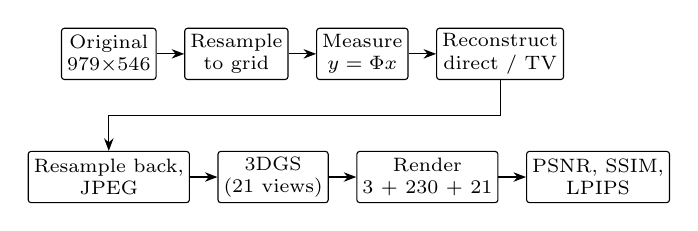
\begin{tikzpicture}[node distance=3.5mm, every node/.style={font=\scriptsize}, box/.style={draw, rounded corners=1pt, align=center, minimum height=6.5mm, inner sep=2pt}, arr/.style={-{Stealth[length=1.6mm]}}]
\node[box] (a) {Original\\979$\times$546};
\node[box, right=of a] (b) {Resample\\to grid};
\node[box, right=of b] (c) {Measure\\$y=\Phi x$};
\node[box, right=of c] (d) {Reconstruct\\direct / TV};
\node[box, below=9mm of a] (e) {Resample back,\\JPEG};
\node[box, right=of e] (f) {3DGS\\(21 views)};
\node[box, right=of f] (g) {Render\\3 + 230 + 21};
\node[box, right=of g] (h) {PSNR, SSIM,\\LPIPS};
\draw[arr] (a)--(b); \draw[arr] (b)--(c); \draw[arr] (c)--(d);
\draw[arr] (d.south) -- ++(0,-4.5mm) -| (e.north);
\draw[arr] (e)--(f); \draw[arr] (f)--(g); \draw[arr] (g)--(h);
\end{tikzpicture}
\caption{Experimental flow. Metrics compare every render with the \emph{original} images. The control skips the measurement step; the baseline skips the whole SPC branch.}
\label{fig:flow}
\end{figure}

\subsection{Measurement model and grids}
Let $x\in\mathbb{R}^{N}$ be a vectorized channel on an $H\times W$ grid, $N=HW$. The camera measures
\begin{equation}
y=\Phi x+n,\qquad \Phi\in\mathbb{R}^{K\times N},\quad r=K/N,
\label{eq:meas}
\end{equation}
with $K=\mathrm{round}(rN)$ and $r\in\{5,10,25,50\}\,\%$. All patterns are made orthonormal ($\Phi\Phi^\top=I$) and are
separable, $\Phi=(A\otimes B)$ restricted to $K$ rows, so $\Phi$ is never stored and is applied with fast transforms.
Hadamard requires power-of-two sides. We use a $256\times512$ grid (main experiment, 131\,072 pixels, 25\,\% of the 534\,534
pixels of an image) and a $512\times1024$ grid (524\,288 pixels, 98\,\%, 2D only and 3D in Sec.~\ref{sec:3d512}).
The aspect ratio of the grid (2.0) differs slightly from that of the images (1.79); the distortion is undone when
resampling back and is part of the control. Resampling to the grid uses area averaging, and back to the image size
bicubic interpolation.

\subsection{Patterns}
\textbf{Hadamard (sequency order).} Rows of the Hadamard matrix are sorted by number of sign changes (sequency) and the 2D
coefficients $(u,v)$ are visited from low to high normalized frequency $u/H+v/W$; the first $K$ are measured.
\textbf{Hadamard (cake-cutting).} The same basis, but coefficients sorted by the number of connected regions of the
pattern, $(u+1)(v+1)$ \cite{yu2019cake}. \textbf{Random binary.} Pixels are permuted with a fixed seed, a Hadamard
transform is applied, and $K$ coefficients are drawn at random; the constant (DC) pattern is always measured, because
without it the mean level is undetermined and TV cannot recover it (a first test without DC gave about 6\,dB).
The resulting patterns are $\pm1$ with a random spatial structure. A dense i.i.d.\ Bernoulli matrix would need
1.7\,GB at 5\,\% and 17\,GB at 50\,\% (1 bit per entry) at $512\times1024$. \textbf{DCT.} A 2D DCT-II in zig-zag order; it is
not binary and serves as a reference in 2D only. A real DMD shows only $\{0,1\}$ masks, so $\pm1$ patterns are obtained
with two complementary patterns (differential measurement); here the $\pm1$ patterns are simulated directly.

\subsection{Reconstruction}
\textbf{Direct:} $\hat x=\Phi^\top y$, the minimum-norm least-squares solution (zeros for unmeasured coefficients).
\textbf{TV:} $\hat x=\arg\min_x\frac12\|\Phi x-y\|_2^2+\lambda\,\mathrm{TV}(x)$ with FISTA (step 1, because
$\Phi\Phi^\top=I$), the TV proximal by Chambolle's algorithm (20 inner iterations), 100 outer iterations and
$\lambda=0.003$. The value of $\lambda$ was chosen with a sweep over $\{0.001,0.003,0.01,0.03\}$ on a view that is not among
the 24 used (000130), for Hadamard and random at 5 and 25\,\%: 0.003 was the best or within 0.2\,dB of the best in all
four cases. The same $\lambda$ is used for all ratios and for both grids; it was not re-validated for $512\times1024$.

\subsection{Detector noise}
The detector model adds Poisson shot noise, Gaussian read noise and $b$-bit quantization,
$y_i=Q_b\!\left(\mathrm{Pois}(\gamma|y_i|)/\gamma+\mathcal N(0,\sigma^2)\right)$ with the sign restored. It is switched off
in all reported experiments except one check (Sec.~\ref{sec:order}), where $\gamma=10^9$ photons, $\sigma=10^{-5}$ of
$\max|y|$ and $b=16$.

\subsection{Data, views and 3DGS training}
We use the Truck scene (251 images of 979$\times$546, COLMAP PINHOLE model of 1957$\times$1091 whose intrinsics are scaled to
the real image size). We take 24 equispaced views (by file name); the test views are positions 4, 12 and 20 of that
selection (000044, 000131, 000218) and the other 21 train. The initial point cloud is the COLMAP one, computed with all 251
views, and it is the same in all conditions. Training uses gsplat 1.5.3 with a compact trainer based on gsplat's
\texttt{simple\_trainer}: default learning rates and \texttt{DefaultStrategy} densification, loss
$0.8\,\mathrm{L1}+0.2(1-\mathrm{SSIM})$, spherical-harmonics degree 3, black background, full resolution, 3000 and 7000
iterations (30\,000 only for baseline and control). Each run is independent.

\subsection{Metrics}
PSNR (range 1, on RGB), SSIM (Gaussian window 11$\times$11, $\sigma=1.5$, per channel) \cite{wang2004ssim} and LPIPS-VGG
\cite{zhang2018lpips} are computed with a single function for all conditions, always at full resolution (979$\times$546)
and against the original image, never against a degraded one.

\subsection{Compute and reproducibility}
All runs used one NVIDIA GeForce RTX 4060 Laptop GPU (8\,GB, driver 571.96) on Windows 11 Home. The 3DGS experiments and the
2D reconstruction ran inside WSL2 (Ubuntu 24.04) with Python 3.12, CUDA toolkit 12.8 and gsplat 1.5.3
(\texttt{TORCH\_CUDA\_ARCH\_LIST}=8.9). The additional 2D timing and pattern-order checks of Sec.~\ref{sec:order} and
Sec.~\ref{sec:time} ran natively on Windows with Python 3.11.14 and PyTorch 2.11.0+cu128. Seed 449 fixes the views, patterns,
noise, initialization and training order. gsplat kernels use atomic additions, so two runs with the same seed can differ
slightly. Everything is driven by YAML configurations (\texttt{configs/}) and a command-line tool; the code is at
\url{https://github.com/fralfaro/spc-gs}.

\section{2D Results}
\label{sec:2d}
All values are means over the 24 views, against the original images. Table~\ref{tab:psnr2d} gives the PSNR on both grids
and Fig.~\ref{fig:2dmetrics} the three metrics. The control (resampling only) gives 27.22\,dB on $256\times512$ and
38.00\,dB on $512\times1024$; it is the ceiling of each grid.

\begin{table}[t]
\caption{2D PSNR (dB), Truck, mean of 24 views. Control: 27.22\,dB ($256\times512$), 38.00\,dB ($512\times1024$).}
\label{tab:psnr2d}
\centering
\footnotesize
\setlength{\tabcolsep}{3pt}
\begin{tabular}{lcccc|cccc}
\toprule
 & \multicolumn{4}{c|}{$256\times512$} & \multicolumn{4}{c}{$512\times1024$}\\
Pattern, method & 5 & 10 & 25 & 50 & 5 & 10 & 25 & 50 \\
\midrule
Hadamard, direct & 20.63 & 21.89 & 23.92 & 25.92 & 23.17 & 25.04 & 28.48 & 33.12 \\
Hadamard, TV & 21.52 & 22.89 & 24.87 & 26.33 & \textbf{24.54} & 26.72 & 30.54 & \textbf{34.39} \\
Random, direct & 12.65 & 12.93 & 13.87 & 15.82 & 12.68 & 13.00 & 14.03 & 16.24 \\
Random, TV & 20.35 & 21.89 & 24.39 & 26.12 & 23.21 & 25.49 & 29.74 & 33.71 \\
DCT, direct & 21.61 & 22.89 & 24.91 & 26.43 & 24.62 & 26.79 & 30.92 & \textbf{35.11} \\
DCT, TV & \textbf{21.80} & \textbf{23.18} & \textbf{25.17} & \textbf{26.49} & \textbf{24.99} & \textbf{27.31} & \textbf{31.33} & 34.99 \\
\bottomrule
\end{tabular}
\end{table}

\begin{figure*}[t]
\centering
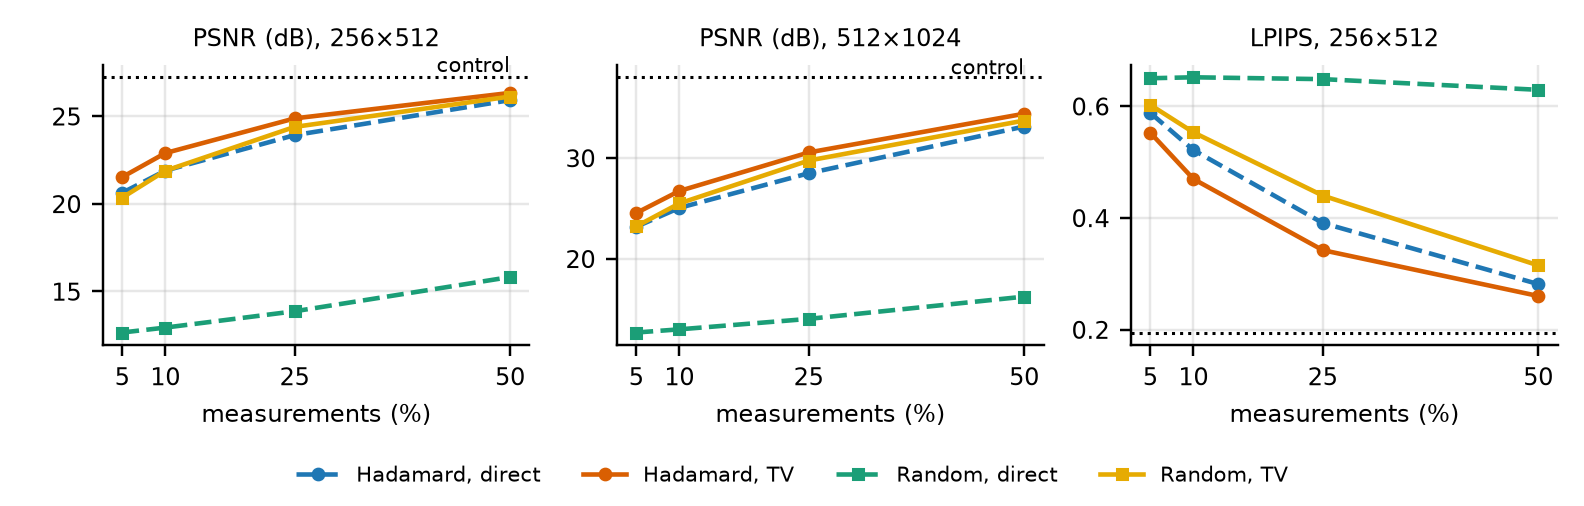
\includegraphics[width=\textwidth]{figs_spc/fig_2d_metrics.png}
\caption{2D quality versus measurement ratio on Truck (mean of 24 views). Left and center: PSNR on the two grids; right: LPIPS
on $256\times512$. Dotted line: control (resampling only, no SPC).}
\label{fig:2dmetrics}
\end{figure*}

\textbf{Quality falls monotonically with fewer measurements.} With Hadamard and TV on $256\times512$, the loss with respect to
the control is 5.70, 4.33, 2.35 and 0.89\,dB at 5, 10, 25 and 50\,\%. The grid is the dominant limit: the same method on
$512\times1024$ reaches 34.39\,dB at 50\,\% because its ceiling is 10.8\,dB higher.

\textbf{TV always helps.} With Hadamard, TV improves the direct reconstruction by 0.89, 1.00, 0.95 and 0.41\,dB on
$256\times512$ and by 1.37, 1.68, 2.06 and 1.27\,dB on $512\times1024$.

\textbf{Random patterns need regularization.} The direct reconstruction of random patterns is unusable (12.65 to 15.82\,dB on
$256\times512$): the unmeasured part spreads over the whole image as noise (Fig.~\ref{fig:visual}). With TV it reaches
20.35 to 26.12\,dB and approaches Hadamard at high ratios (0.21\,dB below at 50\,\%, 1.17\,dB below at 5\,\% on
$256\times512$). On $512\times1024$ the gap to Hadamard with TV is 1.33, 1.23, 0.80 and 0.68\,dB.

\textbf{Hadamard and DCT are close.} DCT is within 1\,dB of Hadamard on $256\times512$; with direct reconstruction at
$512\times1024$ it is better (35.11 against 33.12\,dB at 50\,\%). DCT is not binary, so it cannot be shown on a DMD without
bit-plane tricks, and it is only a reference here.

\begin{figure*}[t]
\centering
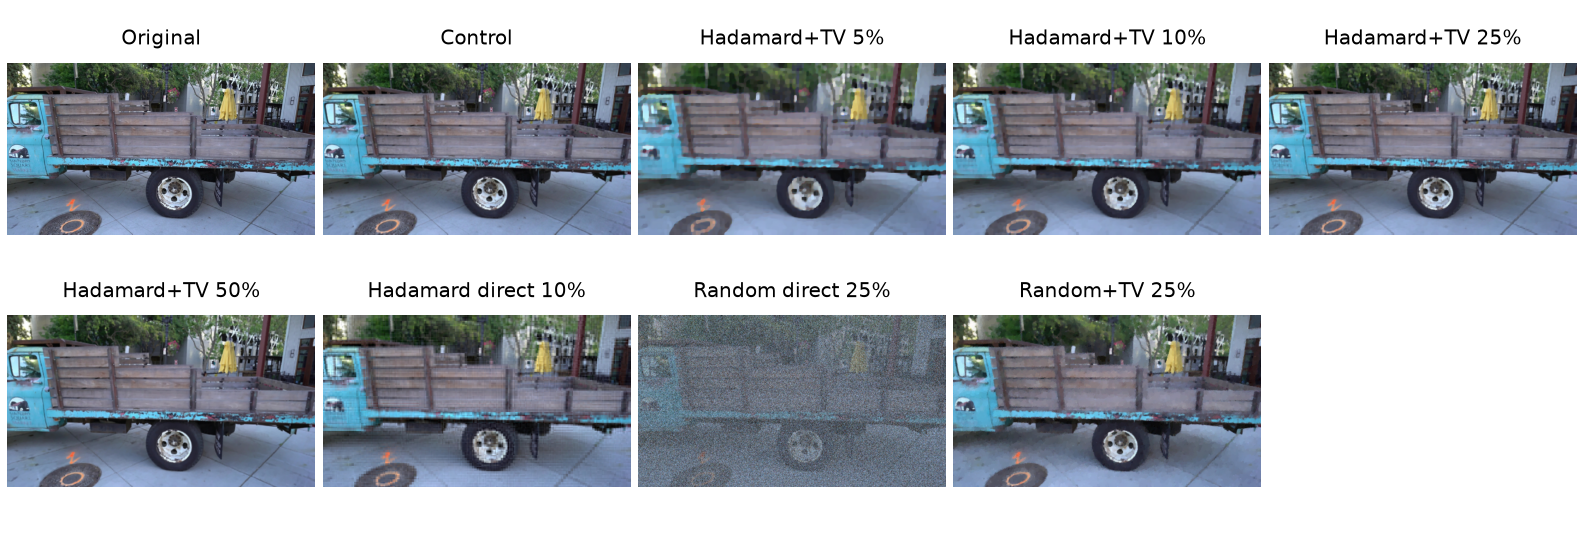
\includegraphics[width=\textwidth]{figs_spc/fig_2d_visual.png}
\caption{Training view 000208 of Truck ($256\times512$ grid). Hadamard with TV loses detail on thin structures at 5\,\%
and recovers the wooden slats and the wheel from 25\,\%; random patterns with direct reconstruction give noise.}
\label{fig:visual}
\end{figure*}

\subsection{Hadamard ordering and noise check}
\label{sec:order}
Because the cake-cutting and the sequency order are different measurement sets, we compared them on $512\times1024$,
all 24 views (Table~\ref{tab:order}). The sequency order is equal or better, by 0.0 to 0.6\,dB, with the largest advantage
at low ratios. Adding the noise model above ($10^9$ photons, $\sigma=10^{-5}$, 16 bits) changed the PSNR of the
cake-cutting order by at most 0.12\,dB, so at these noise levels the detector is not the limiting factor. Because we use the
sequency order in all other experiments, this choice is supported by the data but it is a small effect.

\begin{table}[t]
\caption{Hadamard ordering, 2D PSNR (dB), $512\times1024$, 24 views, no noise.}
\label{tab:order}
\centering
\footnotesize
\begin{tabular}{lcccc}
\toprule
Order, method & 5 & 10 & 25 & 50 \\
\midrule
Sequency, direct & 23.17 & 25.05 & 28.48 & 33.12 \\
Cake-cutting, direct & 22.81 & 24.74 & 28.46 & 32.89 \\
Sequency, TV & 24.54 & 26.72 & 30.54 & 34.39 \\
Cake-cutting, TV & 23.94 & 26.06 & 30.00 & 33.96 \\
\bottomrule
\end{tabular}
\end{table}

\subsection{Why the control matters}
An earlier internal report gave about 38\,dB for the control, which does not match the 27.22\,dB of the main grid. A one-factor
analysis (24 views) shows the cause: with a $512\times1024$ grid, which keeps 98\,\% of the pixels, the control is 38.0\,dB;
with $256\times512$, which discards 75\,\% of them, it is 27.2\,dB. The JPEG at quality 100 costs only 0.02 to 0.14\,dB, and
evaluating at the grid resolution instead of the full resolution would give a misleadingly high 35.21\,dB. This is why every
condition is evaluated at full resolution and why the control is always reported.

\section{3D Results with Gaussian Splatting}
\label{sec:3d}
\subsection{Test views, extended views and training views}
Table~\ref{tab:3d} reports the PSNR of the 7000-iteration models on three evaluation sets, and Fig.~\ref{fig:3dtest} the
three metrics on the test views. We discuss them in order of reliability.

\begin{table*}[t]
\caption{3DGS, 7000 iterations, $256\times512$ grid, seed 449. PSNR (dB) against the original images on the 3 test views, on
230 held-out views, and on the 21 training views. Baseline (original images): 17.72 / 19.40 / 32.51. Control: 18.25 / 19.48 / 26.63.}
\label{tab:3d}
\centering
\footnotesize
\setlength{\tabcolsep}{3.5pt}
\begin{tabular}{lcccc|cccc|cccc}
\toprule
 & \multicolumn{4}{c|}{Test (3 views)} & \multicolumn{4}{c|}{Held-out (230 views)} & \multicolumn{4}{c}{Training (21 views)}\\
Pattern, method & 5 & 10 & 25 & 50 & 5 & 10 & 25 & 50 & 5 & 10 & 25 & 50 \\
\midrule
Hadamard, direct & 17.18 & 17.18 & 17.79 & 18.08 & 17.77 & 18.18 & 18.90 & 19.27 & 20.63 & 21.89 & 23.86 & 25.66 \\
Hadamard, TV & 17.81 & 17.90 & 17.90 & 18.07 & 18.26 & 18.70 & 19.18 & \textbf{19.38} & 21.48 & 22.80 & 24.67 & 25.90 \\
Random, direct & 12.13 & 12.21 & 12.49 & 13.41 & 12.31 & 12.41 & 12.82 & 13.97 & 12.75 & 13.04 & 14.03 & 16.08 \\
Random, TV & 17.27 & 17.43 & 18.05 & 18.16 & 17.53 & 18.30 & 19.01 & 19.40 & 20.32 & 21.83 & 24.19 & 25.73 \\
\bottomrule
\end{tabular}
\end{table*}

\begin{figure*}[t]
\centering
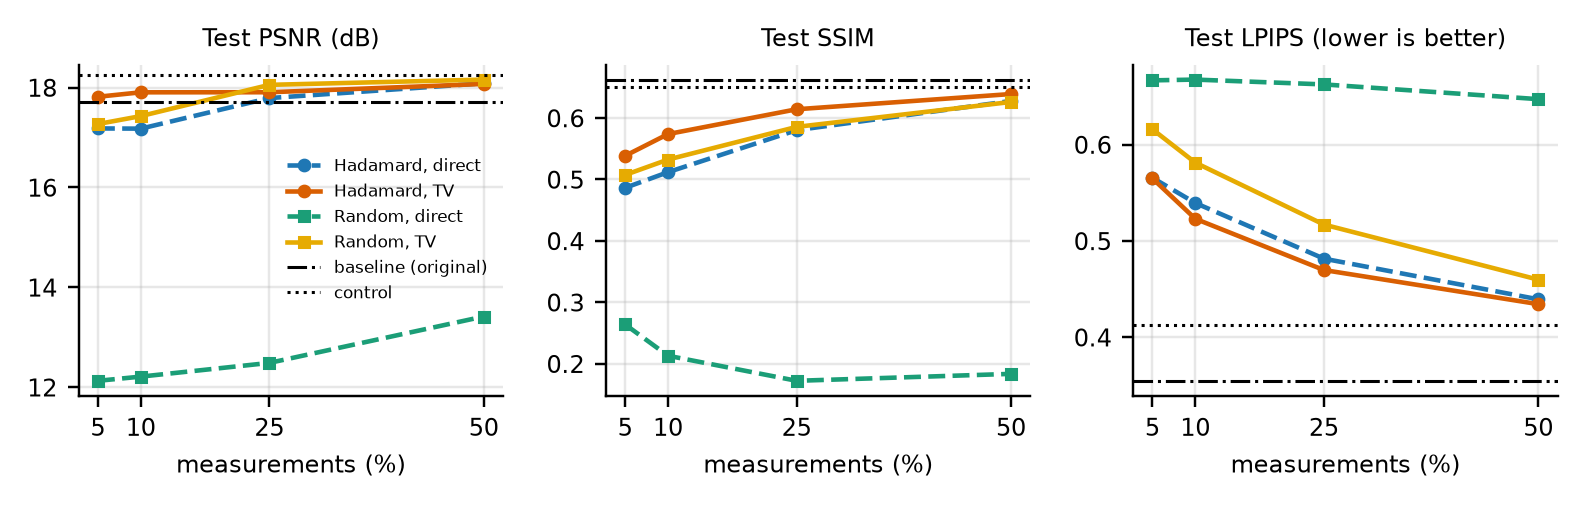
\includegraphics[width=\textwidth]{figs_spc/fig_3d_test.png}
\caption{3DGS (7000 iterations, $256\times512$ grid) on the three test views: PSNR, SSIM and LPIPS against the original images.}
\label{fig:3dtest}
\end{figure*}

\textbf{Test views (3 views): PSNR hardly separates the conditions.} Except for random with direct reconstruction, every
condition falls between 17.18 and 18.57\,dB (7000 and 3000 iterations together), and the control and some SPC conditions
exceed the baseline (17.72\,dB). With only three views this is not conclusive: a seed analysis (seeds 449, 450, 451, 3000
iterations, five conditions) shows a standard deviation of 0.09 to 0.12\,dB on the test PSNR, and of at most 0.05\,dB on the
training PSNR. Pairwise comparisons with 95\,\% intervals over the per-view differences ($n=3$) are conclusive for PSNR in
only 17 of 42 pairs at 7000 iterations (31 of 42 for SSIM and 36 of 42 for LPIPS). SSIM and LPIPS do order the conditions:
the baseline has the best SSIM and LPIPS, and Hadamard (both methods) and random with TV improve monotonically with the ratio.

\textbf{Held-out views (230): the measurement budget matters.} The 230 views that were not used to train any model give a
cleaner ordering (Table~\ref{tab:3d}). Hadamard with TV rises from 18.26\,dB at 5\,\% to 19.38\,dB at 50\,\%, which equals the
baseline (19.40\,dB) and is close to the control (19.48\,dB). Random with TV reaches the same 19.40\,dB at 50\,\%, while random
with direct reconstruction stays at 12.3 to 14.0\,dB. In SSIM and LPIPS the baseline remains better (SSIM 0.732, LPIPS 0.302
against 0.677 and 0.410 for Hadamard with TV at 50\,\%).

\textbf{Training views: 3DGS inherits the 2D degradation.} On the 21 training views the model reproduces almost exactly the
2D loss. For example, Hadamard with TV at 7000 iterations gives 21.48\,dB at 5\,\% (2D: 21.52) and 25.90\,dB at 50\,\%
(2D: 26.33). Relative to the baseline (32.51\,dB), the loss is 5.9\,dB because of the grid alone (control) and 11.0\,dB for
Hadamard with TV at 5\,\%. Fig.~\ref{fig:2d3d} shows that points lie on the diagonal: 3DGS neither repairs nor amplifies the
degradation of the input views.

\begin{figure}[t]
\centering
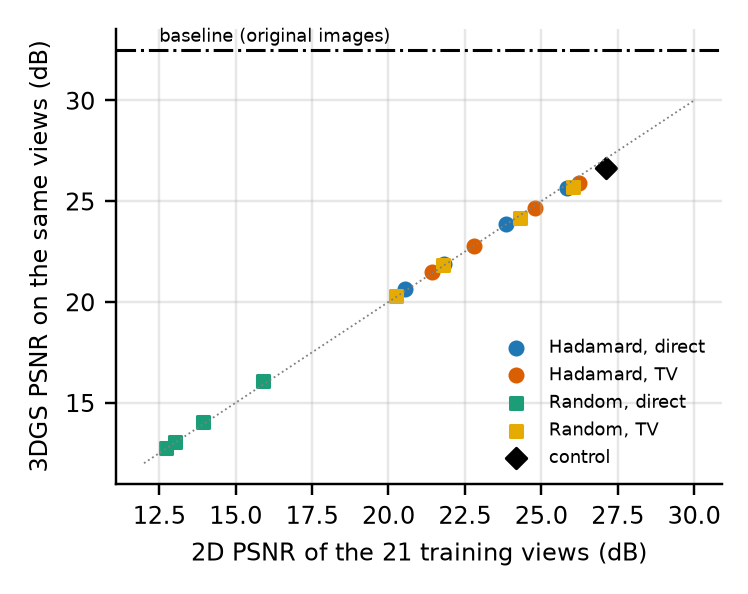
\includegraphics[width=0.9\columnwidth]{figs_spc/fig_2d_to_3d.png}
\caption{2D PSNR of the training views against the PSNR of the 3DGS render of the same views (7000 iterations,
$256\times512$ grid). The dotted line is $y=x$.}
\label{fig:2d3d}
\end{figure}

\textbf{Iterations and over-fitting.} The baseline fits the training views increasingly well (28.81, 32.51 and 40.23\,dB at
3000, 7000 and 30\,000 iterations) but its test PSNR falls (17.97, 17.72 and 17.20\,dB; SSIM 0.676, 0.662, 0.619), which is
consistent with over-fitting to 21 views. The control is limited by the grid on training views (25.90, 26.63 and 27.04\,dB).
In the SPC conditions the change from 3000 to 7000 iterations is at most 0.55\,dB on the training views, because they have
already fitted their degraded images.

\textbf{Qualitative test renders.} Test renders (Fig.~\ref{fig:renders}) show floaters and blurred patches on the ground and
streaks in the background in all conditions, including the baseline, which explains why the test PSNR separates them poorly.
Pixels without Gaussians (accumulated opacity $<0.5$) are few (0.8 to 2.2\,\% of the image) but have the largest mean absolute
error (0.16 to 0.24 against 0.06 to 0.11 over the whole image). The error is lower where more training cameras see the point,
but the relation is not monotonic, so ``poorly observed regions'' is only a partial explanation.

\begin{figure*}[t]
\centering
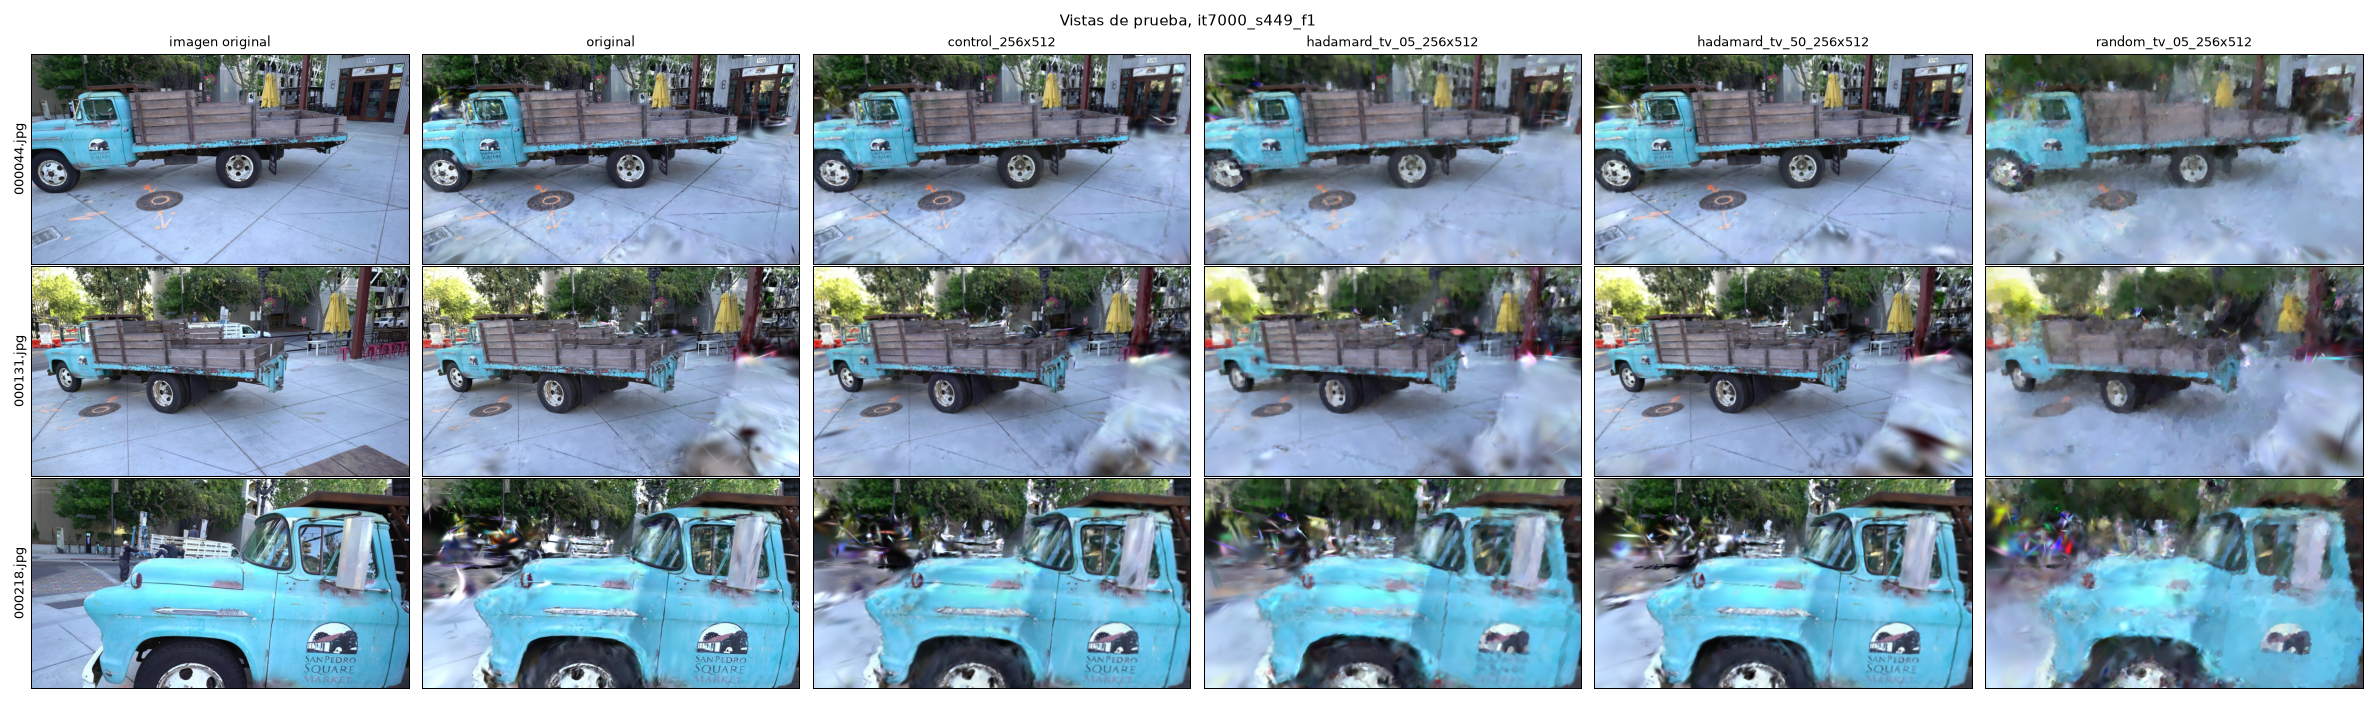
\includegraphics[width=\textwidth]{../../results/figuras/comparacion_prueba_it7000_s449_f1.png}
\caption{Test renders (7000 iterations). Columns: original image, baseline, control, Hadamard with TV at 5\,\% and 50\,\%,
random with TV at 5\,\%.}
\label{fig:renders}
\end{figure*}

\subsection{Reference check of the baseline}
The original 3DGS paper reports 23.5\,dB, SSIM 0.840 and LPIPS 0.209 on Truck at 7000 iterations \cite{kerbl2023}, versus
17.72\,dB, 0.662 and 0.355 for our baseline. The numbers are not comparable and this is \emph{not} a validation: that protocol
trains on most of the 251 views with the official implementation, while we train on 21 views with a compact trainer on gsplat
and evaluate on three test views at full resolution. What the comparison between conditions needs is that all conditions use the
same pipeline, which they do. A validation with the official protocol remains open.

\section{3D Results on a $512\times1024$ Grid}
\label{sec:3d512}
\todo{fill with the 512x1024 3DGS results (job running at the time of writing)}

\section{Time and Memory}
\label{sec:time}
Table~\ref{tab:time} summarizes the cost. The measurements were taken on the RTX 4060 Laptop (8\,GB).

\begin{table}[t]
\caption{Cost on the RTX 4060 Laptop (8\,GB), per view for 2D and per run for 3DGS.}
\label{tab:time}
\centering
\footnotesize
\setlength{\tabcolsep}{3pt}
\begin{tabular}{lll}
\toprule
Stage & Setting & Time\\
\midrule
2D, direct & $256\times512$, $512\times1024$ & $\le$ 7 ms / view \\
2D, TV (100 it.) & $256\times512$ & 0.99--1.27 s / view \\
2D, TV (100 it.) & $512\times1024$, Hadamard & 1.69--1.75 s / view \\
3DGS 3000 it. & all conditions & 63--90 s / run \\
3DGS 7000 it. & all conditions & 146--363 s / run \\
3DGS 30\,000 it. & baseline / control & 3495 s / 1140 s \\
\bottomrule
\end{tabular}
\end{table}

The 2D times are the reconstruction only (synchronized GPU timing, mean of 24 views). The per-condition times saved in the
result files (7.8 to 10.9\,s for direct and 29 to 36\,s for TV, for 24 views) also include image reading, saving and metrics,
so they are not comparable to the per-view reconstruction times. One condition shows 10\,024\,s in that column; we treat it
as an outlier (it is not reproducible by the reconstruction time above) and we did not investigate its cause.
In 3D, one 3000-iteration run took 1213\,s (Hadamard direct 10\,\%) against 63 to 90\,s for the rest, with normal metrics; we
attribute it to the machine (probably power saving) and did not repeat it.

The number of Gaussians depends strongly on the input. The baseline grows from 0.78 M (3000 it.) to 1.36 M (7000 it.) and
2.49 M (30\,000 it.); SPC conditions with TV use 0.29 to 0.61 M at 7000 iterations, because TV removes the noise that other
conditions try to fit; random patterns with direct reconstruction need up to 1.89 M Gaussians (50\,\%, 7000 it.) because they
try to fit the noise. Peak reserved memory was 4.25\,GiB for that run, 3.35\,GiB for the baseline at 7000 iterations and
5.65\,GiB at 30\,000 iterations. The maximum read with \texttt{nvidia-smi} during the whole experiment was 4875\,MiB (it
includes memory used by Windows). A 30\,000-iteration run of the 16 SPC conditions was not done for time (19 to 58 minutes per
run for baseline and control).

\section{Discussion}
\textbf{What the experiments say.} (i) In 2D, the cost of measuring less is clear and smooth, and the grid is a bigger factor
than the ratio on a coarse grid. (ii) A regularizer is worth about 1 to 2\,dB with Hadamard and is essential with random
patterns. (iii) In 3D, a 2D metric predicts the quality of training views almost one to one, but it predicts test quality
poorly with few views, so conclusions about generalization need many held-out views or several seeds. (iv) With a
$256\times512$ grid and 50\,\% of the measurements, the SPC-based models are as good as the baseline on held-out views
(19.38 against 19.40\,dB), which suggests that for this scene the test error is dominated by the sparsity of the 21 views and
not by the photometric quality of the input.

\textbf{Cost.} A TV reconstruction costs about 1 to 1.7\,s per view on a laptop GPU, about 200 to 1000 times the direct one, and
3DGS adds minutes. The time of the SPC itself (the measurement sequence on a real DMD) is not modeled.

\section{Limitations}
\label{sec:limits}
\begin{itemize}
\item One scene (Truck) and one main seed. Differences of a few tenths of a dB may be within the training variability.
\item Only 21 training views, so absolute 3DGS values are lower than published ones; the comparison between conditions is what
the study supports.
\item Three test views (plus 230 held-out views as an extended evaluation); the PSNR on three views is not sensitive.
\item Poses and the initial point cloud come from COLMAP on the original images; a real SPC would not have them, so the 3D results
are an optimistic bound.
\item The views are already captured images, not an optical acquisition: measurements inherit the dataset's JPEG and blur, and
they are in sRGB, not linear radiance. A DMD with $\pm1$ patterns is simulated directly. The scene is assumed static.
\item Noise is off in the reported results; the single noise check changed the PSNR by at most 0.12\,dB.
\item $\lambda=0.003$ was selected on one view and for the $256\times512$ grid; it was not re-tuned for $512\times1024$.
\item The 3DGS trainer is a compact one built on gsplat and its baseline was not validated against the official implementation.
\end{itemize}

\section{Conclusions and Future Work}
Measuring 5\,\% of the coefficients with Hadamard patterns and TV costs 5.70\,dB with respect to the control on a
$256\times512$ grid, and 50\,\% costs 0.89\,dB. TV helps in all cases and is indispensable for random patterns. In 3D, 3DGS
reproduces the 2D degradation on its training views, and on 230 held-out views Hadamard with TV at 50\,\% matches the
baseline, while the PSNR on three test views cannot rank the conditions. Future work: more scenes and seeds, a validation of the
baseline with the official protocol, re-estimating poses with COLMAP on the SPC views, noise in the 3D experiments, training 3DGS
directly against the measurements, and patterns that change between views.

\section*{Use of AI Tools}
Claude Code (Anthropic) was used to review and organize the implementation, run analyses and draft visualizations and text.
The code, the tabulated values and the conclusions were checked by the authors against the executed experiments and the cited
references.

\bibliographystyle{IEEEtran}
\bibliography{references}

\end{document}
